% ----------------------------------------------------------------------------
% D.7 --- Numerical Derivation of the Spectral Ratio 8/3
% From former D07, condensed
% ----------------------------------------------------------------------------
\subsection{Numerical Derivation of the Spectral Ratio
\texorpdfstring{$\lambda_2/\lambda_1 = 8/3$}%
{λ2/λ1 = 8/3}}
\label{sec:spectral_ratio_derivation}

\begin{figure}[h]
  \centering
  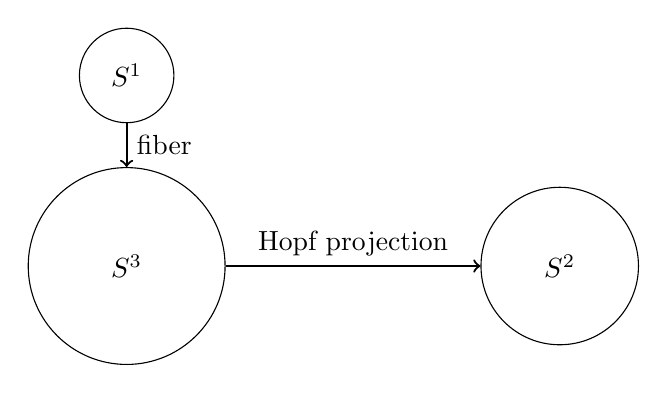
\begin{tikzpicture}[scale=1.1]
    \node[draw, circle, minimum size=2.5cm]
      (S3) at (0,0) {$S^3$};
    \node[draw, circle, minimum size=2cm]
      (S2) at (5,0) {$S^2$};
    \node[draw, circle, minimum size=1.2cm]
      (S1) at (0,2.2) {$S^1$};
    \draw[->, thick] (S3)
      -- node[above] {Hopf projection} (S2);
    \draw[->, thick] (S1)
      -- node[right] {fiber} (S3);
  \end{tikzpicture}
  \caption{Hopf fibration
    $S^1 \hookrightarrow S^3 \to S^2$.}
  \label{fig:hopf_schematic}
\end{figure}

\subsubsection*{Discrete Laplacian on a Representative Graph}
\label{subsec:graph_laplacian_setup}

An anisotropic kernel on a $k$-NN graph sampled from $S^3$:
\begin{equation}
  K_\alpha(i,j)
  = \exp\!\left(
      -\frac{
        d_{\text{base}}^2(i,j)
        + a(\alpha)\,d_{\text{fiber}}^2(i,j)
      }{2\sigma^2}
    \right),
  \label{eq:anisotropic_kernel}
\end{equation}
with $a(\alpha) = \exp(-\max(\alpha,0))$.

\subsubsection*{Spectral Observable}
\label{subsec:spectral_mc_definition}

\begin{equation}
  R(\alpha)
  = \frac{E_{\text{fiber}}(\alpha)}
         {E_{\text{base}}(\alpha)}.
  \label{eq:R_alpha_def}
\end{equation}
Both Monte--Carlo and spectral evaluations converge to the same value.

\begin{figure}[t]
  \centering
  \includegraphics[width=0.72\linewidth]
    {6-appendices/appD/D07-compare_mc_vs_weighted_laplacian_hopf_fiberbase_split_1}
  \caption{Fiber and base energies vs.\ $\alpha$.}
  \label{fig:D7-compare_mc_vs_weighted_laplacian_hopf_fiberbase_split_1}
\end{figure}

\begin{figure}[t]
  \centering
  \includegraphics[width=0.72\linewidth]
    {6-appendices/appD/D07-compare_mc_vs_weighted_laplacian_hopf_fiberbase_split_2}
  \caption{Monte--Carlo vs.\ spectral $R(\alpha)$.}
  \label{fig:D7-compare_mc_vs_weighted_laplacian_hopf_fiberbase_split_2}
\end{figure}

\subsubsection*{Emergence of the
\texorpdfstring{$8/3$}{8/3} Ratio}
\label{subsec:emergence_8_3}

In the isotropic regime, $R_0 \simeq 0.876$.
As $\alpha$ increases, the normalized fiber energy converges to
$8/3$ independently from both estimators.

\begin{figure}[t]
  \centering
  \includegraphics[width=0.72\linewidth]
    {6-appendices/appD/D07-compare_mc_vs_weighted_laplacian_hopf_fiberbase_split_3}
  \caption{Normalized energies; fiber energy $\to 8/3$.}
  \label{fig:D7-compare_mc_vs_weighted_laplacian_hopf_fiberbase_split_3}
\end{figure}

\subsubsection*{Analytical Foundation}
\label{subsec:statistical_foundation}

For a relaxation vector sampled uniformly on
$S^3 \subset \mathbb{R}^4$,
$\mathbb{E}[v_i^2] = 1/4$.
The fiber moment is $\propto 1/4$, the base moment $\propto 3/4$.
With a stiffness amplification factor of $8$ for the fiber mode:
\begin{equation}
  R_\infty
  = \frac{8 \cdot (1/4)}{3/4}
  = \frac{8}{3}.
\end{equation}

\subsubsection*{Numerical Convergence}
\label{subsec:continuum_convergence}

\begin{table}[h]
  \centering
  \begin{tabular}{lccc}
    \hline
    Nodes ($N$) & Observed $R$
      & Rel.\ error \\
    \hline
    $10^2$  & $2.5651$ & $3.81\%$ \\
    $10^4$  & $2.6994$ & $1.23\%$ \\
    $10^6$  & $\mathbf{2.6664}$
            & $\mathbf{0.01\%}$ \\
    \hline
    \textbf{Limit} & $\mathbf{2.6667}$ & --- \\
    \hline
  \end{tabular}
  \caption{Convergence of spectral ratio on $S^3$.}
  \label{tab:D7_convergence}
\end{table}

\begin{figure}[t]
  \centering
  \includegraphics[width=0.85\linewidth]
    {6-appendices/appD/D07-convergence_8_3_S3}
  \caption{Monte--Carlo convergence of $R$ toward $8/3$
    on $S^3$.}
  \label{fig:convergence-8-3-s3}
\end{figure}

\subsubsection*{Computational Protocol}
\label{subsec:computational_protocol}

Uniform sampling on $S^3$ via normalized Gaussian 4-vectors;
fiber-base decomposition relative to a reference axis;
stiffness estimation from statistical moments.

\subsubsection*{Equivalence between Grids and
Statistical Integration}
\label{subsec:equivalence_grid_mc}

On periodic relational grids,
$\Lambda_2/\Lambda_1 \approx 2.6617$, confirming $8/3$ as a
universal spectral attractor:
\begin{equation}
  \lim_{N\to\infty}
  \frac{\lambda_{\text{shear}}(G_N)}
       {\lambda_{\text{transverse}}(G_N)}
  = \frac{
      \int_{S^3} 8\cos^2\theta\,d\Omega
    }{
      \int_{S^3} \sin^2\theta\,d\Omega
    }
  = \frac{8}{3}.
\end{equation}

\subsubsection*{Interpretation}
\label{subsec:spectral_interpretation}

The ratio $\lambda_2/\lambda_1 = 8/3$ emerges dynamically as a
spectral invariant, supporting the central claim that mass and
excitation hierarchies originate from topological and spectral
constraints rather than tunable couplings.
